\documentclass[11pt]{article}
\usepackage{amsmath, amssymb, amscd, amsthm, amsfonts}
\usepackage{graphicx}
\usepackage{hyperref}
\usepackage{subfigure}
\usepackage{float}

\oddsidemargin 0pt
\evensidemargin 0pt
\marginparwidth 40pt
\marginparsep 10pt
\topmargin -20pt
\headsep 10pt
\textheight 8.7in
\textwidth 6.65in
\linespread{1.2}

\title{Digital Bubble Level}
\author{Vladislav Pomogaev - 26951160}
\date{September 27, 2021}

\newcommand{\rr}{\mathbb{R}}

\newcommand{\al}{\alpha}
\DeclareMathOperator{\conv}{conv}
\DeclareMathOperator{\aff}{aff}

\begin{document}

\maketitle

\section{Introduction}
This device forms a digital "bubble level"; also called a "spirit level". It can be helpful in aligning things horizontally.
\begin{figure}[H]
    \centering
    \subfigure[]{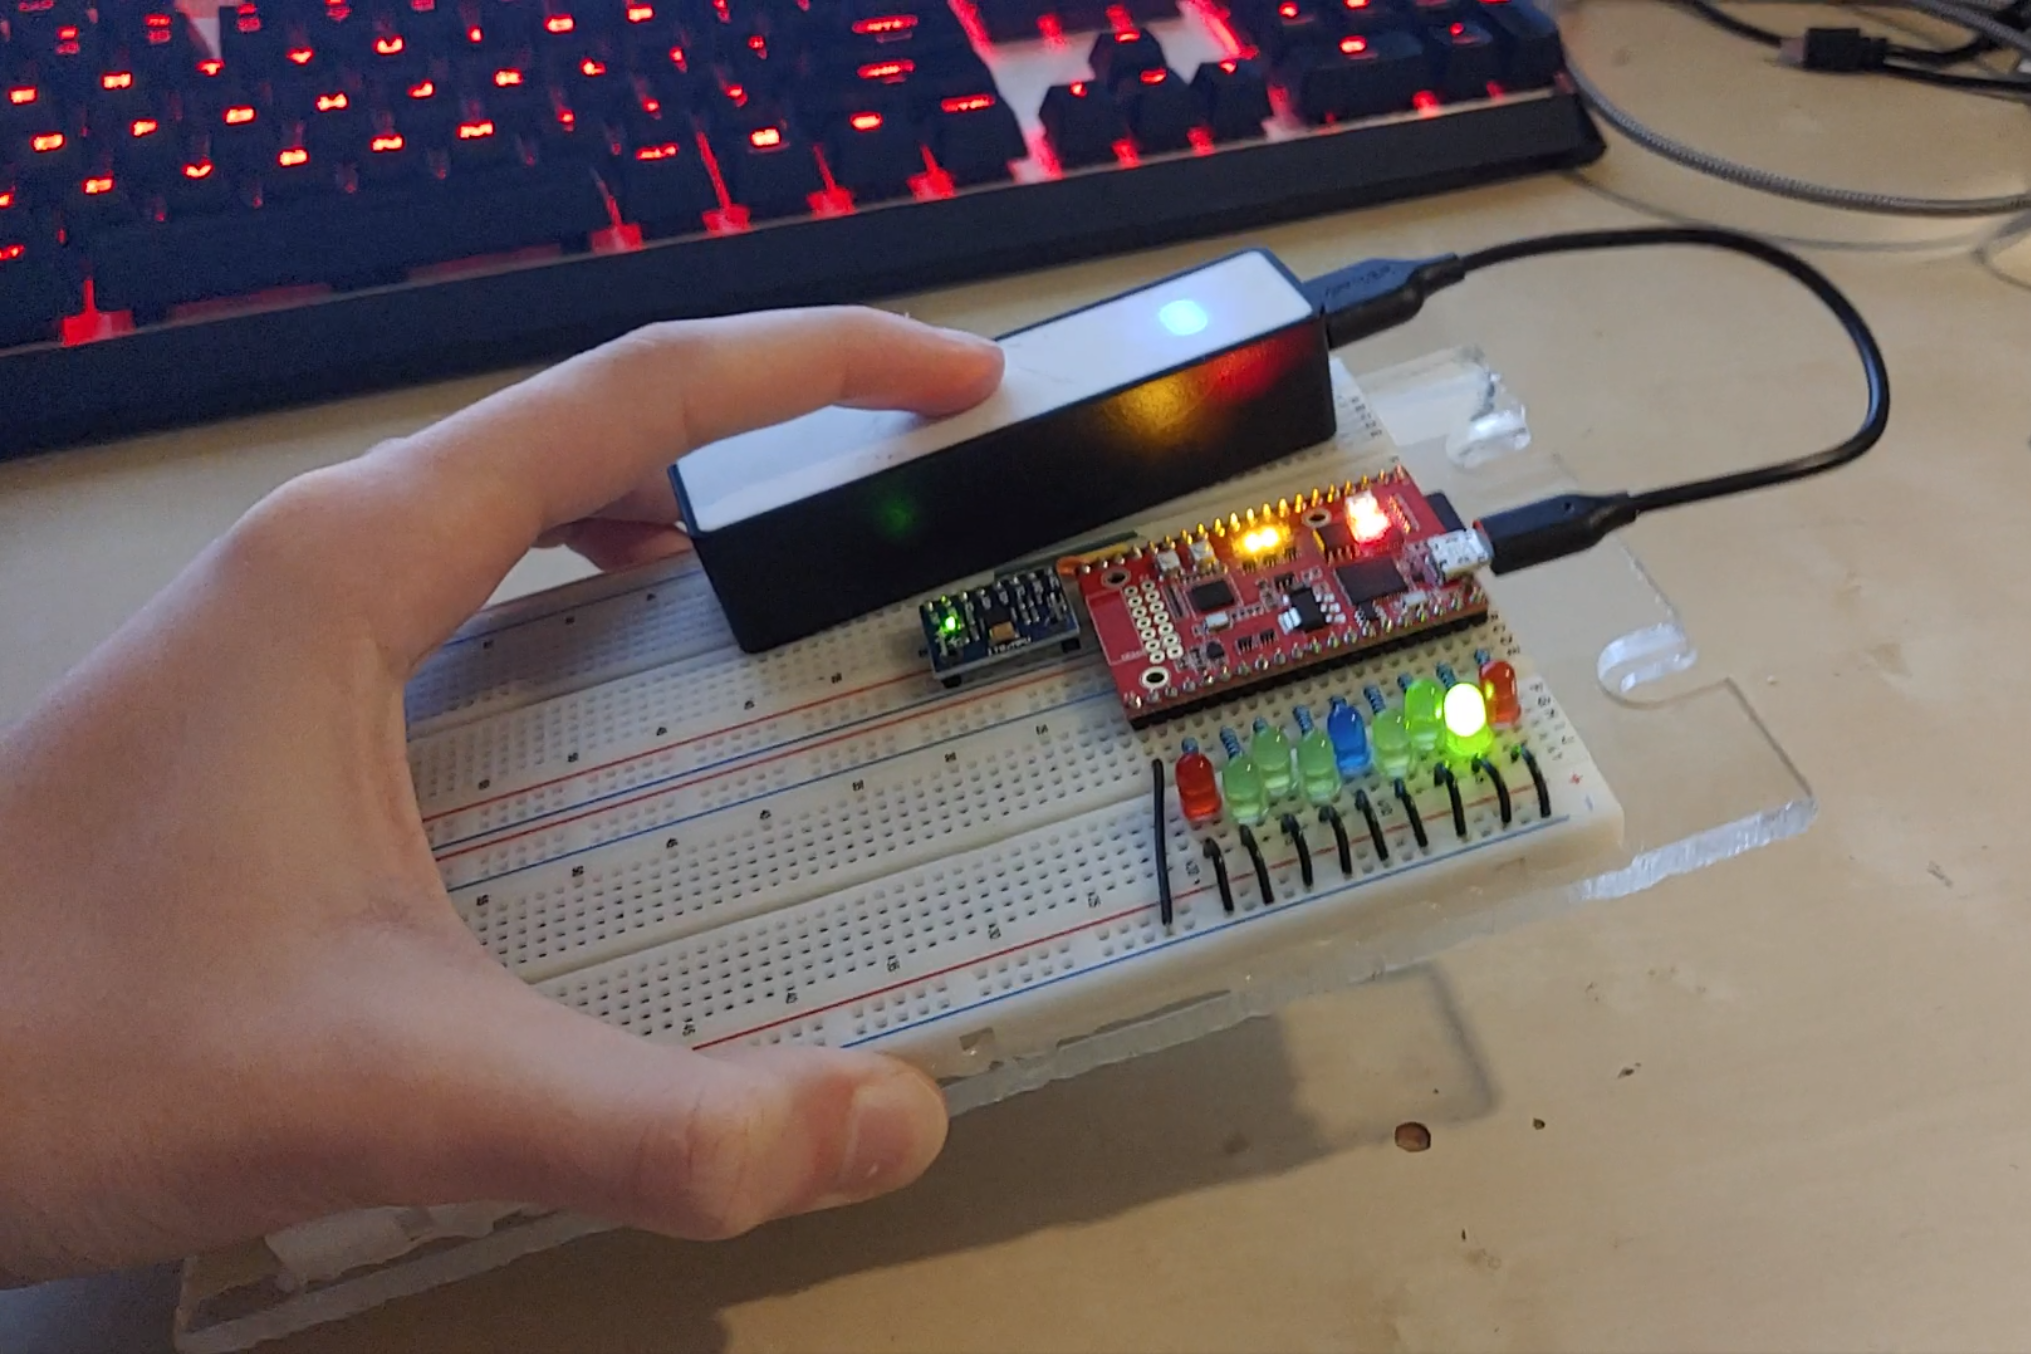
\includegraphics[width=0.32\textwidth]{tilt_1.png}} 
    \subfigure[]{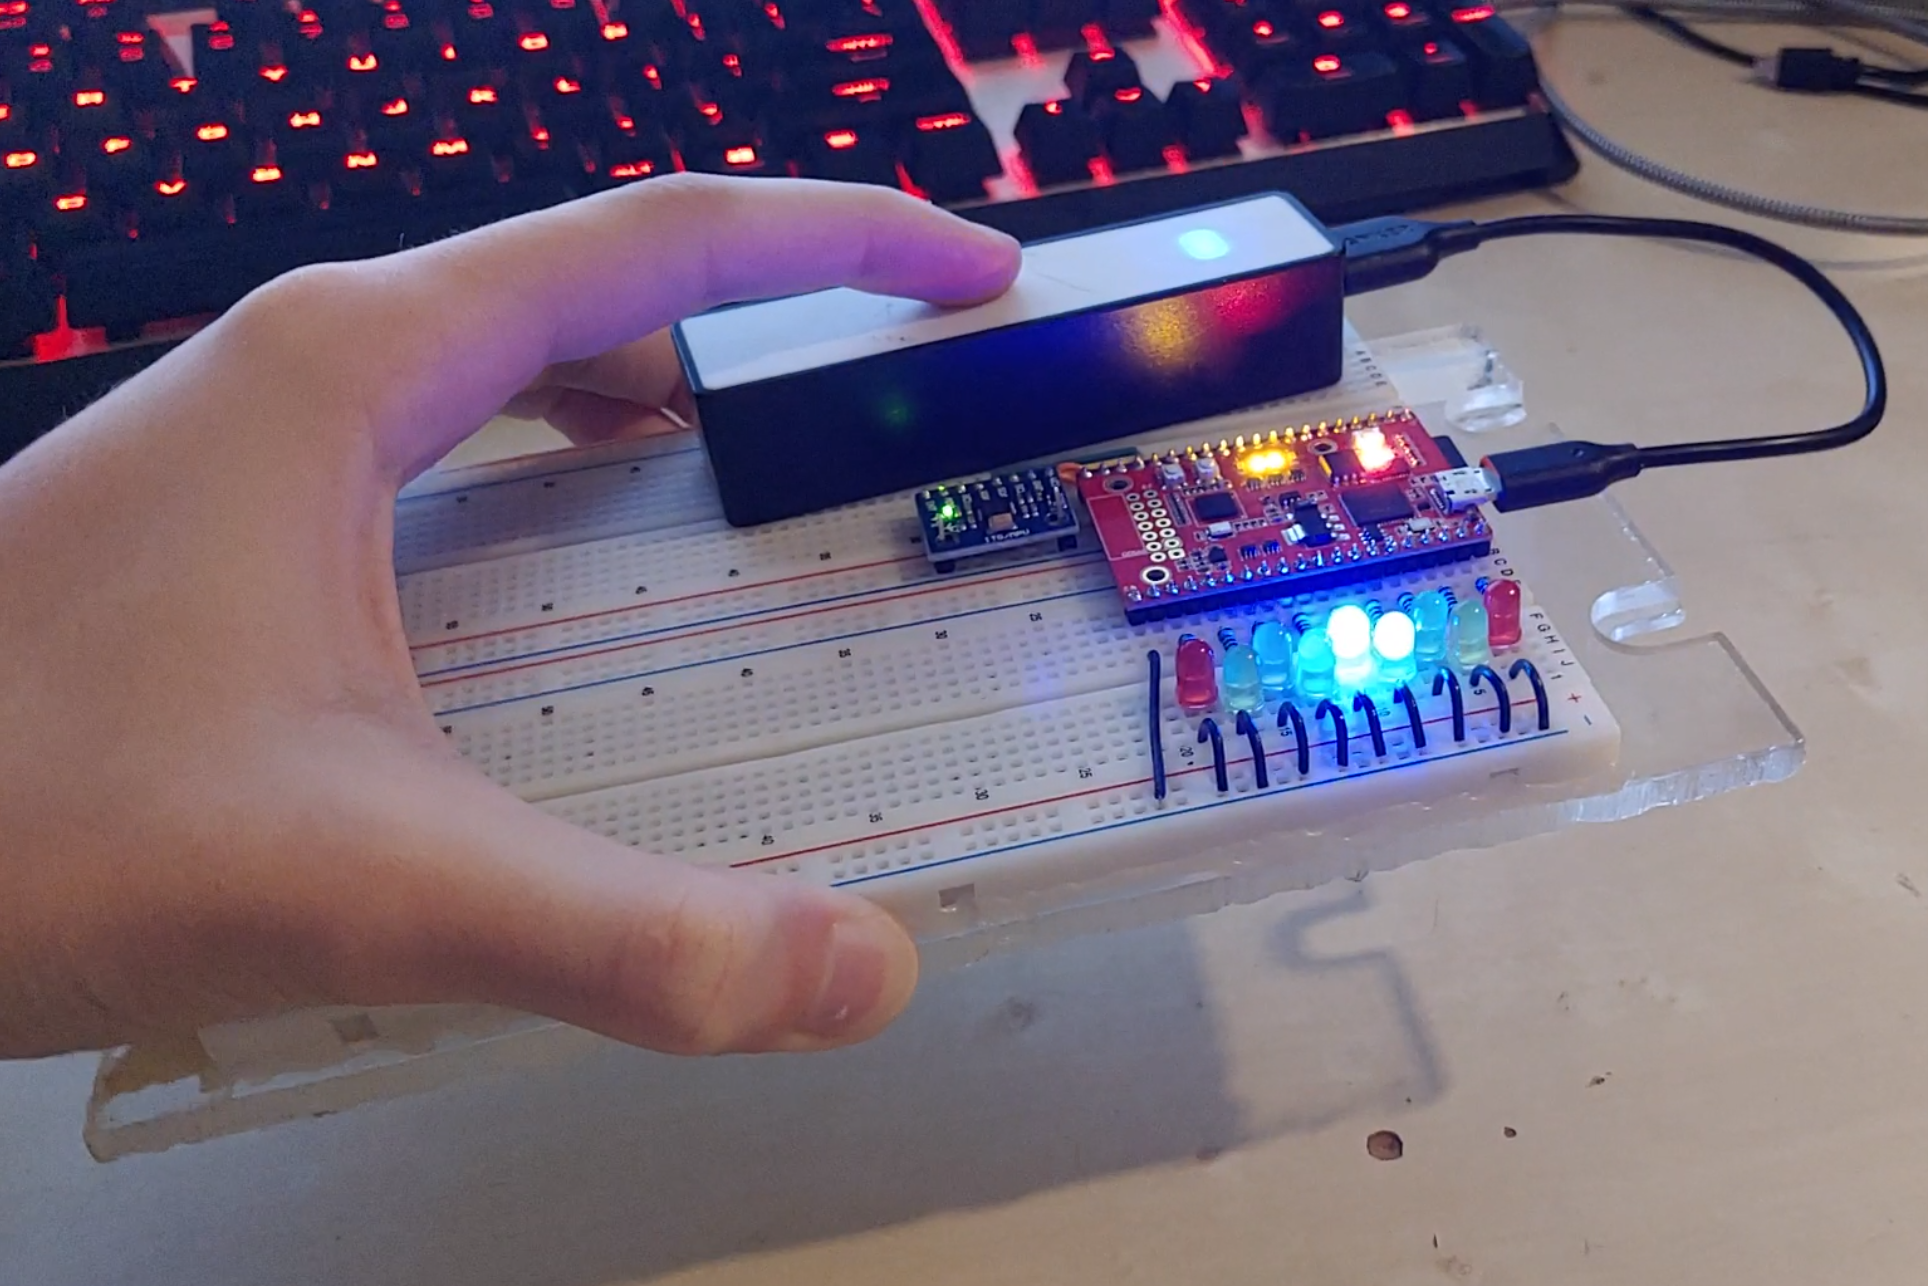
\includegraphics[width=0.32\textwidth]{tilt_3.png}} 
    \subfigure[]{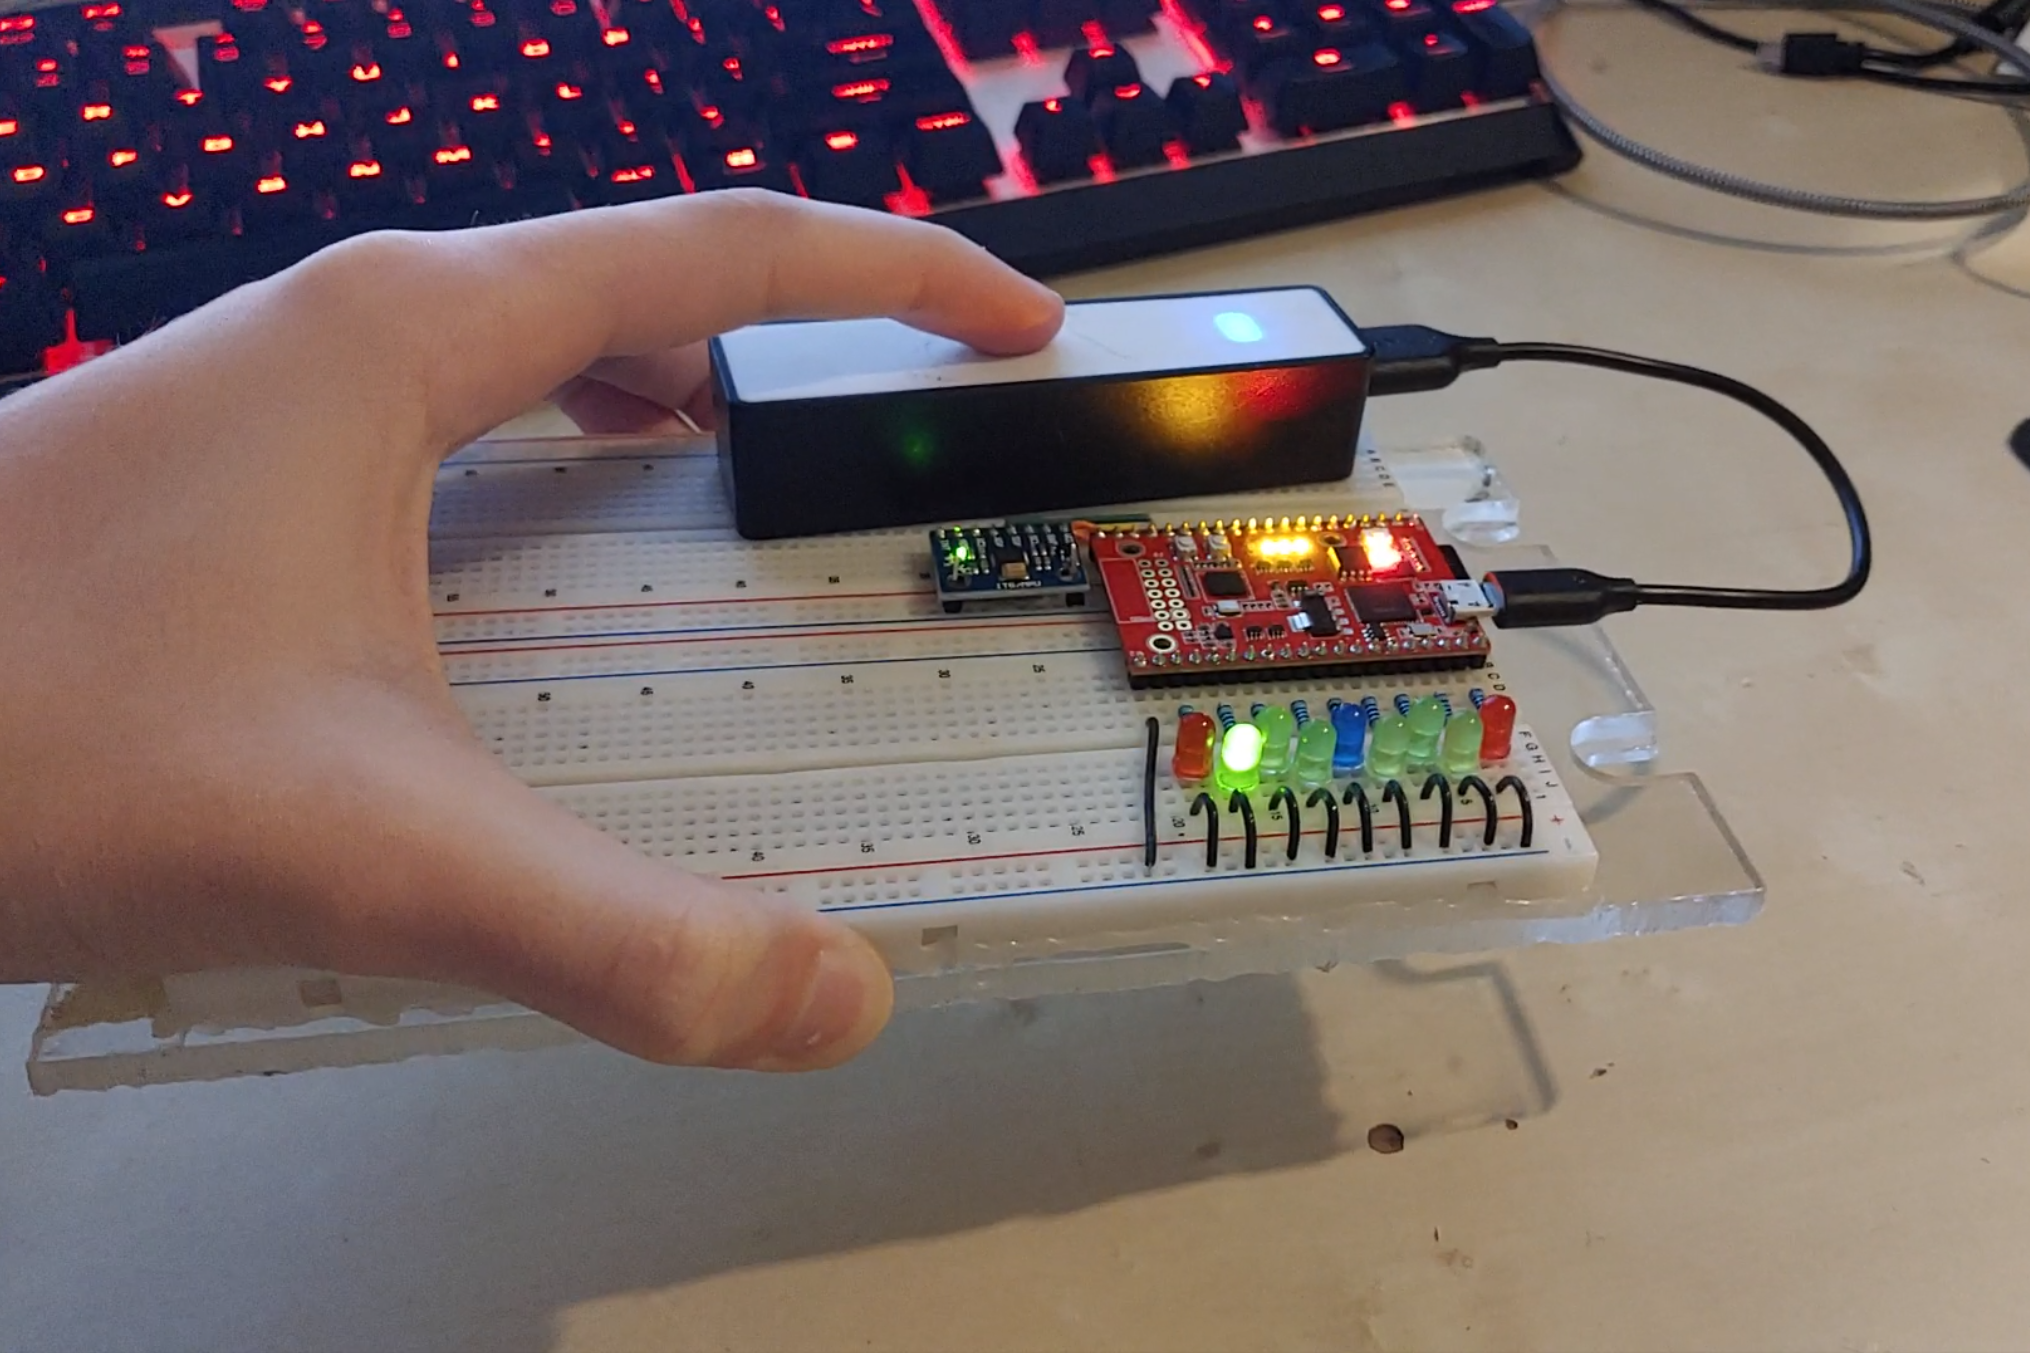
\includegraphics[width=0.32\textwidth]{tilt_2.png}}
    \caption{Photo stills of the device in action. When you tilt the device to the left as in a), the LEDs to the right light up. As you tilt the device more to the right, the lit LED moves from right to left as in b) and c). When level, the blue center LED lights up.}
    \label{fig:foobar}
\end{figure}

This project consists of a synthesised Verilog design running on an Efinix Xyloni FPGA development board. An accelerometer (MPU-6050) and 9 LEDs are connected to this board.

The Verilog design consists of an FSM (Finite State Machine), and an I\textsuperscript{2}C controller IP block from Efinix. The FSM can send commands to the accelerometer through the I\textsuperscript{2}C controller, which acts as the master. Upon reset, the FSM wakes the accelerometer by writing to a register. Then, in a loop, the FSM requests the acceleration measured in one axis from the accelerometer, and converts the acceleration to a grey-code-like signal which is then output to the LEDs. All of this is done using the communication protocol established by the I\textsuperscript{2}C controller. The FSM must request data in the correct format, provide slave address, data, command byte, and number of data bits, wait for response, and check for errors during every read and write command.

\section{Introduction}


\end{document}